A range query is a database operation that retrieves all the records that lies in a range. In this project, we perform range query on 2-dimensional data only. In addition, we only consider a range query where the range is defined as a rectangle. Under these assumptions, a range query can be formalised as a query $\mathcal{Q}(\boldsymbol{l}, \boldsymbol{u})$ where $l,u\in\mathbb{R}^2$.

\begin{mscexample}
	For example, assume we have the points
	$$
	[(1,2), (3,4), (3.5, 4), (5,6)]
	$$
	and the range query $\mathcal{Q}((2,3), (5,5))$, as shown below:
	
	\begin{minipage}[t]{\linewidth}
	\centering
   	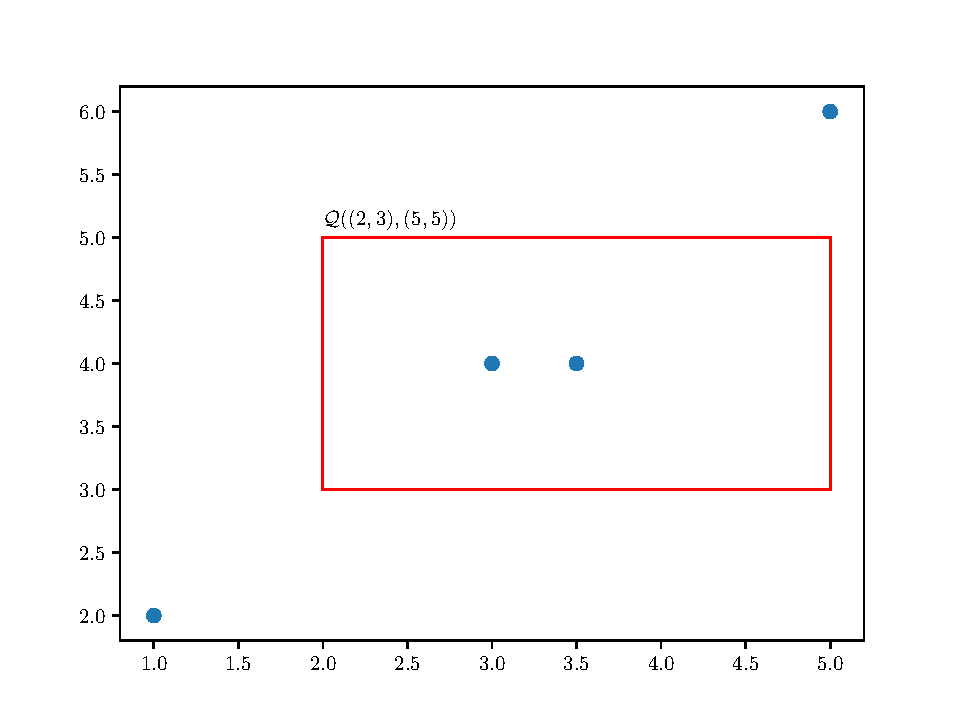
\includegraphics[width=10cm]{graphs/implementation/queries/range_query.pdf}
   	\label{fig:range_query_demo}
   	\captionof{figure}{A Range Query Example where $\mathcal{Q}(\boldsymbol{l}, \boldsymbol{u})=\mathcal{Q}((2,3),(5,5))$}
	\end{minipage}
	
In this example, the range query should return the points that lies inside the red rectangle, i.e. $((3,4), (3.5, 4))$.

\end{mscexample}

\subsubsection{Range Query with $K$D-Tree}

\begin{figure}[htp]
    \centering
    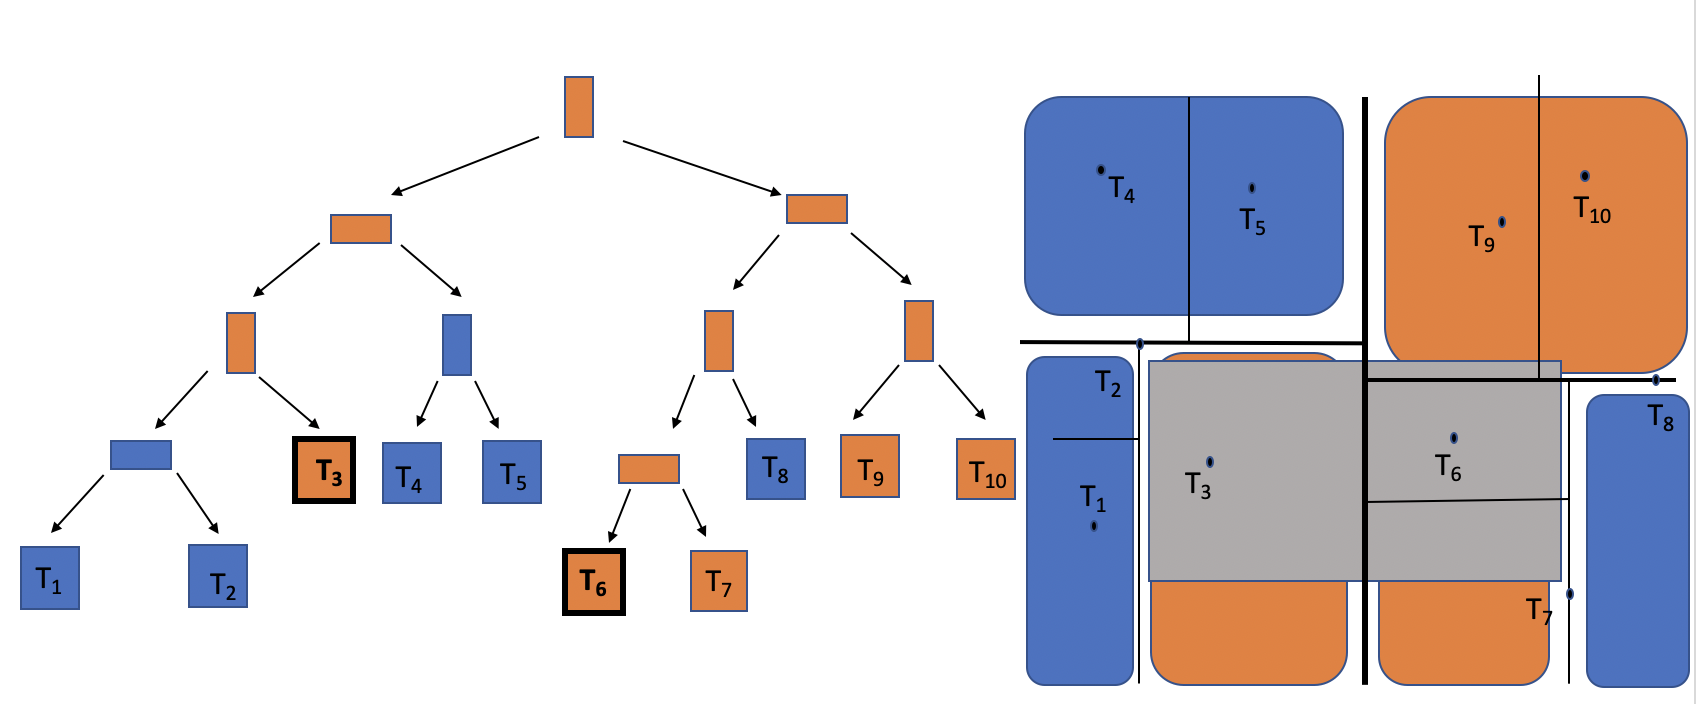
\includegraphics[width=1.0\textwidth]{graphs/KD_Tree_Range_Query_Algorithm.png}
    \caption{$K$D-Tree for Range Query Algorithm (Orange color are the visited points and blue color are the points not visited) 
    1) Tree representation of points. \\
    2) Subdivision of space into cells.(Orange color are the visited cells and blue color are the cells not visited) 
    }
    \label{fig:KD-Tree_for_Range_Query_Algorithm}
\end{figure}


% TODO: THIS ALGORITHM IS STILL NOT COMPLETE, and hard to follow.

\begin{algorithm}[H]
    \SetAlgoLined
    \SetKwInOut{Input}{Input}
    \SetKwInOut{Output}{Output}
    \Input{Lower and Upper bound of query range rectangle $\mathcal{Q}(\boldsymbol{l}, \boldsymbol{u}); [l \in \mathbb{R};u \in \mathbb{R}]$}
    \Output{\texttt{List of Points within query range rectangle($Rectangle$)}}
    \texttt{SEARCH\_RANGE\_QUERY($Rectangle$)}\\
    \eIf{node.leftChild is leaf}
        {
            \If {$cell(v) \subseteq Rectangle$}
                {add all points within cell to list}
            \eIf {$cell(v) \cap Rectangle = \varnothing$}
                {add nothing to list}
            {add all points reported within $cell(v) \cap Rectangle$}
        }
        {
            \texttt{SEARCH\_RANGE\_QUERY($Rectangle$)} //Recursively function is called\\
        }
        
    \texttt{Similarly, steps are repeated for node.rightChild}
    
    \caption{Range Query Algorithm for $K$D-Tree}
    \label{Range_Query_Algorithm_$K$D-Tree}
\end{algorithm}

In algorithm \ref{Range_Query_Algorithm_$K$D-Tree} we first check the root of the tree in the function SEARCH\_RANGE\_QUERY(). We pass the lower and upper bound of the rectangles and check if the point at the root fall within the range rectangle. If point falls within the range then the point is added to the list.
In fig \ref{fig:KD-Tree_for_Range_Query_Algorithm} we see how the space is partitioned on x-axis and y-axis alternatively. The subdivision consists of rectangular regions, called cells (possibly unbounded). Suppose current splitting line is vertical. Let v, w be left and right children nodes. After checking the root, root.leftChild (v) is searched to see if the it is a leaf node. Since v is not a leaf node a decision to traverse the right or left subtree is made by checking it's x-axis, y-axis and split axis. In  fig \ref{fig:KD-Tree_for_Range_Query_Algorithm} we can see that all cells that intersect the range rectangle is checked (highlighted by orange color) and all the cells that are not intersected by the rectangle are pruned and not checked (highlighted in blue). This improves the performance of the range query and hence results in much faster query.


There are two cases in range query search:
\begin{enumerate}
    \item\textbf{Case 1}: When en entire subtree lie within range of rectangle.
    \item\textbf{Case 2}: When only a part of the subtree lie within range of rectangle.
\end{enumerate}

\begin{figure}[htp]
    \centering
    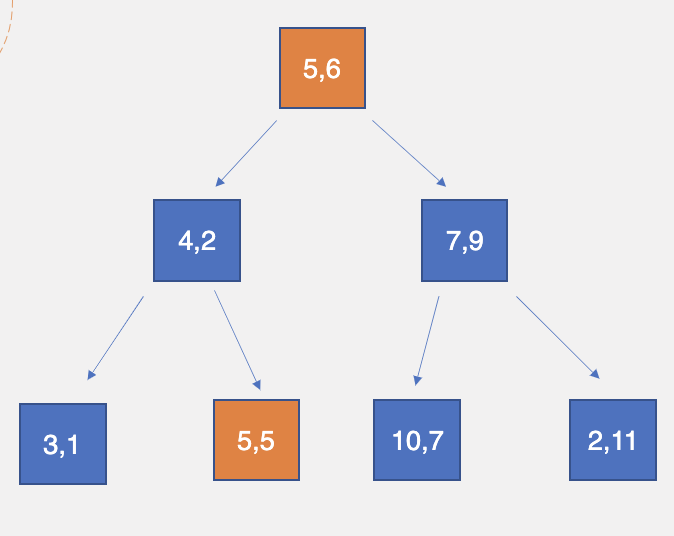
\includegraphics[width=0.4\textwidth]{graphs/Range_Query_Tree.png}
    \caption{$K$D-Tree for Range Query (Case 1)}
    \label{fig:KD-Tree_for_Range Query}
\end{figure}


\begin{figure}[htp]
    \centering
    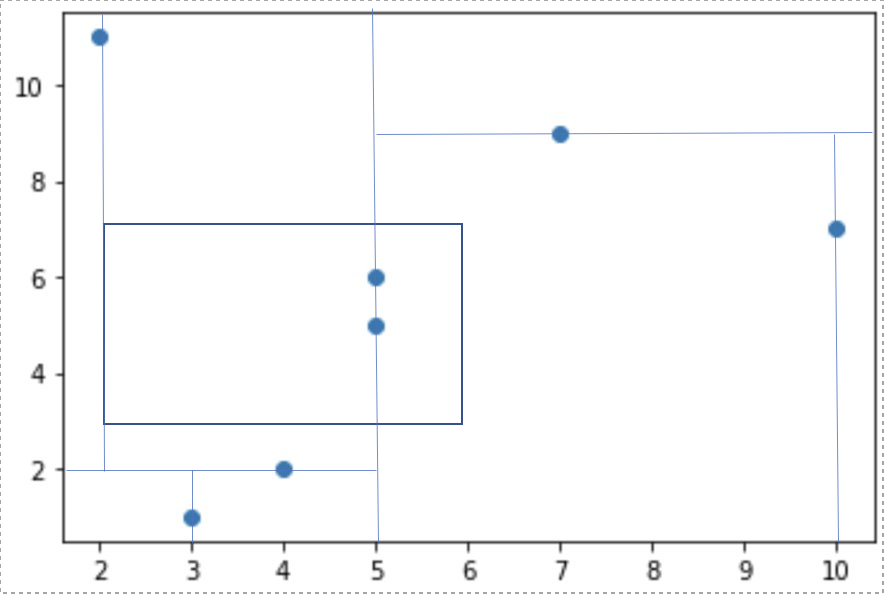
\includegraphics[width=0.6\textwidth]{graphs/Range_Query_plot.png}
    \caption{$K$D-Tree Range Query Plot on 2-dimensional plane (Case 1)}
    \label{fig:KD_Tree_Range_Query_Plot}
\end{figure}


\begin{figure}[htp]
        \centering
        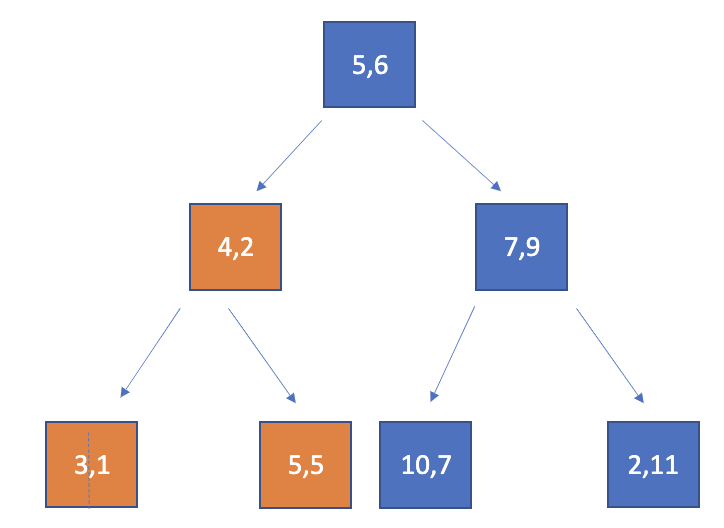
\includegraphics[width=0.4\textwidth]{graphs/Range_Query_Tree_02.png}
        \caption{$K$D-Tree for Range Query (Case 2)}
        \label{fig:KD-Tree_for_Range_Query_Case2}
\end{figure}


\begin{figure}[htp]
    \centering
    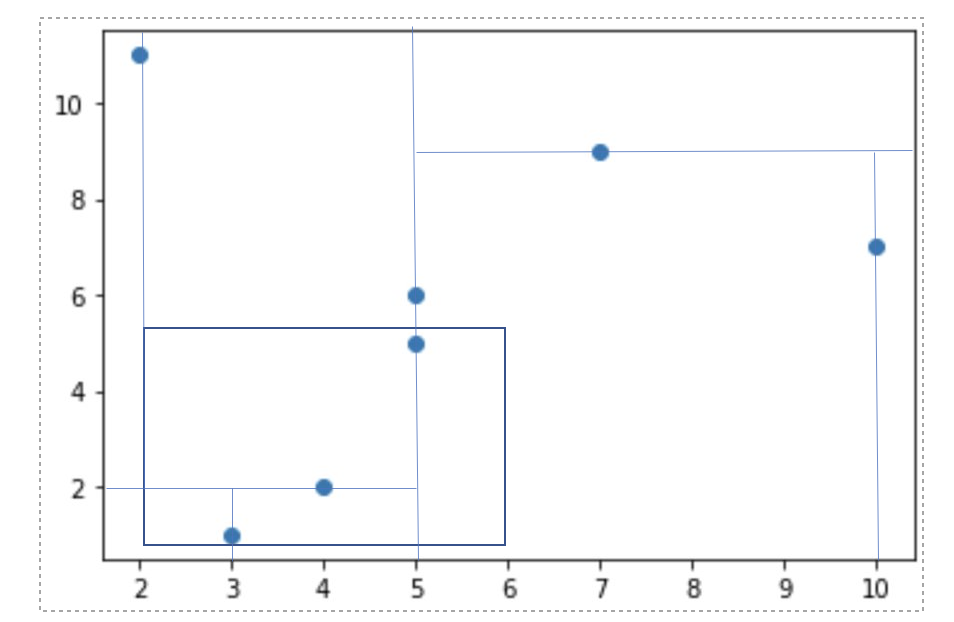
\includegraphics[width=0.6\textwidth]{graphs/Range_Query_plot_02.png}
    \caption{$K$D-Tree Range Query Plot on 2-dimensional plane (Case 2)}
    \label{fig:KD_Tree_Range_Query_Plot_Case2}
\end{figure}

\begin{mscexample}


    \textbf{Case 1} : For example we have a tree with Point list as 

	$$((5,6),(4,2),(7,9),(3,1),(5,5),(10,7),(2,11))$$
	
	 with \textbf{lower bound} = $(2,3)$ and \textbf{upper bound} = $(6,7)$, we will get a tree as is shown in \ref{fig:KD-Tree_for_Range Query}. We can see the points along with range rectangle plotted in \ref{fig:KD_Tree_Range_Query_Plot}. Points $(5,5)$ and $(5,6)$ are returned in the query since they lie within the rectangle as seen in the plot.\\
	Firstly, the root point is checked and since the x-coordinate and y-coordinate both lie within the rectangle bounds i.e., $2 > 5 > 6$ and $3 > 6 > 7$. It is added to the result list.\\
	Secondly, we have to check weather to traverse left or the right of the tree. To do this, we then checks if the x-coordinate of root is greater than or equal to the lower bound x-coordinate of range rectangle. Since the value is larger than lower bound x-coordinate that is $5 > 2$ it will then traverse to the left. In the left, root has leftChild node $(4,2)$ however, here we will check if both the coordinates lie within the rectangle. Since the y-coordinate doesn't lie in the range of the rectangle, this point is not selected i.e., $2 \notin [3,7]$. Similarly, it recursively traverses the tree and checks if the point lies within the bound until it reaches a leaf.\\
	
	\textbf{Case 2} : For example we have a tree with Point list as 

	$$((5,6),(4,2),(7,9),(3,1),(5,5),(10,7),(2,11))$$
	
	with \textbf{lower bound} = $(2,0.5)$ and \textbf{upper bound} = $(6,4.75)$, we will get a tree as shown in \ref{fig:KD-Tree_for_Range_Query_Case2}. We can see the points along with range rectangle plotted in \ref{fig:KD_Tree_Range_Query_Plot_Case2}.Points $(4,2)$, $(3,1)$ and $(5,5)$ are returned in the query since they lie within the rectangle as seen in the plot.\\
	Firstly, the root point is checked and since the y-coordinate both do not lie within the rectangle bounds i.e., $6 \notin [0.5, 4.75]$ it is not added to the list.\\
	Secondly, we will check weather to traverse left or right of the tree. To do this, we then checks if the x-coordinate of root is greater than or equal to the lower bound x-coordinate of range rectangle. Since the value is larger than lower bound x-coordinate that is $5 > 2$ it will then traverse to the left. In the left, root has leftChild node $(4,2)$ and since both the x-coordinate and y-coordinate lie within the range of rectangle it is added to the result list. \\ We will then traverse to both left and then right since all the points in this cell lie within the range of rectangle and hence are added to the list.
\end{mscexample}

\begin{figure*}[t]
    \centering
    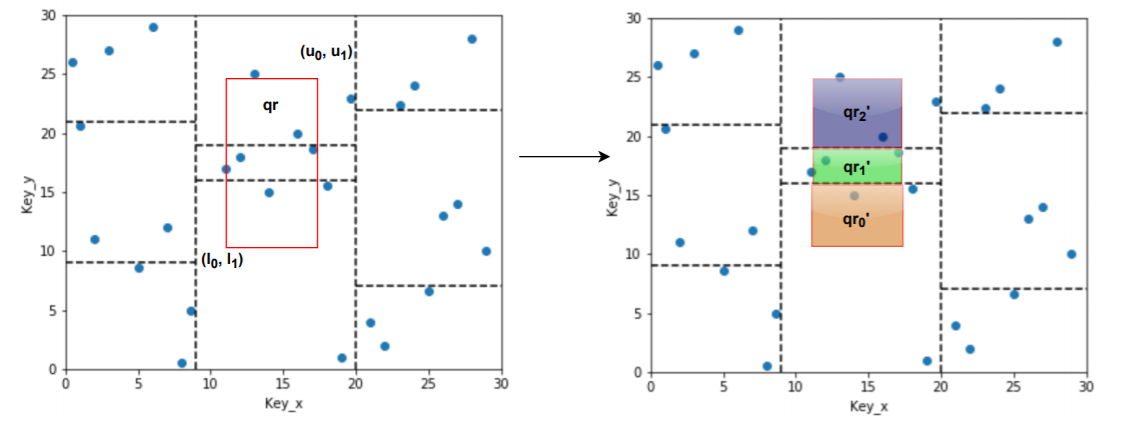
\includegraphics[width=1\textwidth]{graphs/range_query_lisa.png}
    \caption{Range Query Search in Lisa.
    1) Find the cells that overlap with query rectangle qr. \\
    2) Decompose qr into the unions of smaller query rectangles, each of which intersect one only one cell. \\
    3) Find shards corresponding to lower and upper coordinates for each query rectangle, and perform a sequential search. }
    \label{fig:Range_Query_Lisa}
\end{figure*}


\subsubsection{Range Query with LISA}


For a range query $\mathcal{Q}(\boldsymbol{l},\boldsymbol{u})$, we first find the cells that overlap with $\mathcal{Q}$. Then we decompose $\mathcal{Q}$ into the union of smaller query rectangles $\bigcup \mathcal{Q}_i$ such that each smaller query rectangles intersects only one cell, as shown in the Fig. \ref{fig:Range_Query_Lisa}.



 Suppose that $\mathcal{Q}=\bigcup \mathcal{Q}_i$ where $\mathcal{Q}_i=[l_{i_0}, u_{i_o})\times [l_{i_1}, u_{i_1})$, i.e. we have $\mathcal{Q}_i$ representing the $i$th smaller query rectangles of one cell $C_j$.
 
 Then we can calculate the mapped values of $\mathcal{Q}_i$, i.e. $\mathcal{M}(l_{i_0}, l_{i_1})$ and $\mathcal{M}(u_{i_0}, u_{i_1})$. For simplicity, we use $m_l^{(i)}$ and $m_u^{(i)}$ to denote $\mathcal{M}(l_{i_0}, l_{i_1})$ and $\mathcal{M}(u_{i_0}, u_{i_1})$ respectively.
 
After creating corresponding mapped values, we then apply the shard prediction function $\mathcal{SP}(m_{l}^{i})$ and $\mathcal{SP}(m_{u}^{i})$ to predict the shard that could possibly contain keys that lie in the query rectangle $\mathcal{Q}_i$. Then in each shard, we perform a sequential search to find the desired keys. 

